\chapter{Impostazione di seL4}
Come primo approccio per arrivare alla scrittura di questa tesi ho innanzitutto fatto una ricerca sulla letteratura che si trova disponibile riguardo a seL4, nonostante sia poca e principalmente fornita da Trustworthy (TS) stesso comunque sufficiente per avere una conoscenza abbastanza approfondita del microkernel.\\
SeL4 è un sistema open-source dunque lo step successivo è stato quello di scaricare seL4 e sperimentare con mano le funzionalità, ovviamente questo ha richiesto un approfondimento più tecnico e specifico, rispetto a quanto fatto finora, di alcuni aspetti come la gestione della memoria fisica e virtuale, l'IPC ecc. che verranno trattati in questo capitolo.

\section{Prerequisiti}
Come prima cosa ho installato sul mio portatile VirtualBox in quanto come consigliato dalle guide fornite da TS sarebbe ottimale lavorare in ambiente Linux, non avendo una partizione del portatile con Linux ho inizialmente pensato di utilizzare una macchina virtuale così da lasciare inalterato il mio computer e comunque avere a disposizione un sistema operativo Linux su cui lavorare. Andando avanti con il set-up del sistema per iniziare a lavorare su seL4 però ho incontrato una prima difficoltà che è stata lo spazio: purtroppo lo spazio nel portatile non era tantissimo, la macchina virtuale, considerando il sistema operativo e l'installazione dei vari prerequisiti per poter far girare il microkernel, cominciava ad occupare molto spazio, dunque ho dovuto cercare un'alternativa; Per sopperire al problema mi sono procurato un SSD su cui sono andato a copiare la partizione creata in VirtualBox continuando la sperimentazione sul microkernel lavorando sull'SSD esterno collegato via USB.\\
Per lavorare su seL4 è necessario avere installato sul sistema dei programmi che simulino un'architettura su cui farlo girare, per fare ciò è necessario installare delle dipendenze (prerequisiti) cioè compilatori, emulatori software vari e librerie che devono essere installate affinché sia possibile utilizzare seL4.\\
Prima di tutto ho installato Google repo, così da poter clonare i repository git:
\definecolor{codegreen}{rgb}{0,0.6,0}
\definecolor{codegray}{rgb}{0.5,0.5,0.5}
\definecolor{codepurple}{rgb}{0.58,0,0.82}
\definecolor{backcolour}{rgb}{0.95,0.95,0.92}
\lstdefinestyle{mystyle}{
    backgroundcolor=\color{backcolour},   
    commentstyle=\color{codegreen},
    keywordstyle=\color{magenta},
    numberstyle=\tiny\color{codegray},
    stringstyle=\color{codepurple},
    basicstyle=\ttfamily\footnotesize,
    breakatwhitespace=false,         
    breaklines=true,                 
    captionpos=b,                    
    keepspaces=true,                  
    numbersep=5pt,                  
    showspaces=false,                
    showstringspaces=false,
    showtabs=false,                  
    tabsize=2
}

\lstset{style=mystyle}

\begin{lstlisting}[language=bash]
sudo apt-get install repo
\end{lstlisting}
build-essential, cmake, ninja, curl, python e QEMU abbreviazione di Quick EMUlator, un emulatore open-source che permette di emulare un'architettura informatica e che permette di simulare diversi sistemi operativi, in questo caso è fondamentale perchè permette l'esecuzione di seL4:
\begin{lstlisting}[language=bash]
sudo apt-get install build-essential
sudo apt-get install cmake ccache ninja-build cmake-curses-gui
sudo apt-get install libxml2-utils ncurses-dev
sudo apt-get install curl git doxygen device-tree-compiler
sudo apt-get install u-boot-tools
sudo apt-get install python3-dev python3-pip python-is-python3
sudo apt-get install protobuf-compiler python3-protobuf
sudo apt-get install qemu-system-arm qemu-system-x86 qemu-system-misc
pip3 install --user setuptools
pip3 install --user sel4-deps
\end{lstlisting}
Altro componente fondamentale è CAmkES (component architecture for microkernel-based embedded systems), un framework per realizzare velocemente sistemi multiserver affidabili basati su microkernel:
\begin{lstlisting}[language=bash]
pip3 install --user camkes-deps
curl -sSL https://get.haskellstack.org/ | sh
sudo apt-get install haskell-stack
sudo apt-get install clang gdb
sudo apt-get install libssl-dev libclang-dev libcunit1-dev libsqlite3-dev
sudo apt-get install qemu-kvm
\end{lstlisting}
Dopodiché sono passato alle dipendenze per l'installazione di Isabelle (theorem prover) che serve per la verifica automatica di sistemi software e hardware:
\begin{lstlisting}[language=bash]
sudo apt-get install \
    python3 python3-pip python3-dev \
    gcc-arm-none-eabi build-essential libxml2-utils ccache \
    ncurses-dev librsvg2-bin device-tree-compiler cmake \
    ninja-build curl zlib1g-dev texlive-fonts-recommended \
    texlive-latex-extra texlive-metapost texlive-bibtex-extra \
    mlton-compiler haskell-stack repo
\end{lstlisting}
Ancora dipendenze Python e Haskell
\begin{lstlisting}[language=bash]
pip3 install --user --upgrade pip
pip3 install --user sel4-deps

stack upgrade --binary-only
which stack # should be $HOME/.local/bin/stack
stack install cabal-install
\end{lstlisting}
Con questa serie di comandi bash il sistema operativo Linux, per la precisione Ubuntu \textcolor{red}{VERSIONE}, ha tutti i prerequisiti necessari per procedere alla configurazione.

\section{Configurazione}
Lo step successivo è stato quello di recuperare, attraverso repo, la collezione di repository necessari per la verifica di seL4; in particolare contiene il sorgente del kernel, il theorem prover Isabelle/HOL e HOL4 e lo strumento di verifica binaria.
\begin{lstlisting}[language=bash]
mkdir verification
cd verification
repo init -u https://git@github.com/seL4/verification-manifest.git
repo sync
\end{lstlisting}
A questo punto  si avrà quindi una cartella con questa struttura:
\dirtree{%
.1 verification.
.2 HOL4/.
.2 graph-refine/.
.2 isabelle/.
.2 l4v/.
.2 seL4/.
}
Il che indica che l'importazione delle repository è andata a buon fine, quindi possiamo procedere alla configurazione di Isabelle posizionandosi nella cartella \texttt{l4v}:
\begin{lstlisting}[language=bash]
mkdir -p ~/.isabelle/etc
cp -i misc/etc/settings ~/.isabelle/etc/settings
./isabelle/bin/isabelle components -a
./isabelle/bin/isabelle jedit -bf
./isabelle/bin/isabelle build -bv HOL
\end{lstlisting}
Questa serie di comandi bash daranno come risultato:
\begin{itemize}
	\item la creazione di una cartella per le impostazioni utente di Isabelle.
	\item installazione delle impostazione Isabelle per L4.verified \cite{l4v} il rtbj6nmgquale è una repository che contiene formalismi per la verifica di seL4.
	\item download di Scala, Java JDK, PolyML ed altri dimostratori (prover) esterni.
	\item compilazione del Prover IDE (PIDE) jEdit di Isabelle
\end{itemize} 

\section{Avvio di SeL4}
Terminata la prima fase di installazione dei prerequisiti e di configurazione mi sono procurato ciò che servirà poi per eseguire i test delle varie funzionalità di seL4:
\begin{lstlisting}[language=bash]
mkdir seL4test
cd seL4test
repo init -u https://github.com/seL4/sel4test-manifest.git
repo sync
\end{lstlisting}
Con questi comandi si va a creare una directory \texttt{seL4test} al cui interno, attraverso il comando \texttt{repo}, che conterrà tutte le direttive e le librerie necessarie per eseguire i vari test (quindi anche il kernel stesso).\\
Dopodichè è stato necessario creare una cartella \texttt{build-x86} di configurazine per QEMU in modo da indicargli il target su cui eseguire le simulazioni:
\begin{lstlisting}[language=bash]
mkdir build-x86
cd build-x86
../init-build.sh -DPLATFORM=x86_64 -DSIMULATION=TRUE
ninja
\end{lstlisting}
Il comando \texttt{ninja}, che si vedrà spesso a seguire, è un assembler che permette di fare il build di sistemi anche complessi molto velocemente.\\
A questo punto è possibile eseguire il comando \texttt{./simulate} che farà partire la simulazione e dopo una lunga serie di test (IPC, chiamate di sistema, thread...) che appariranno nel terminale, concluderà, se tutto è andato a buon fine, con:\\
\texttt{All is well in the universe}\\
Il che indica che seL4 può essere utilizzato in questo ambiente simulato.
\begin{figure}[h!]
  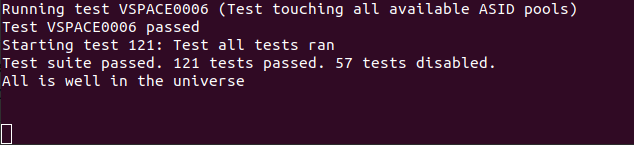
\includegraphics[width=\linewidth]{img/PrimaSimulazione.png}
  \label{fig:Prima simulazione}
\end{figure}

\section{Programmazione con le API livello kernel di seL4}
Una volta che mi sono procurato tutti i prerequisiti necessari e appurato che seL4 può girare senza problemi ho iniziato a prendere familiarità con il sistema seguendo dei tutorial forniti dalla seL4 Foundation che sono programmi semicompleti creati appositamente per sperimentare e far comprendere le funzionalità del sistema, in particolare con le API di seL4. \cite{sel4API}\\
Come ormai già visto più volte sopra ho recuperato l'ambiente per eseguire i tutorial attraverso l'uso di \texttt{repo}:
\begin{lstlisting}[language=bash]
mkdir sel4-tutorials-manifest
cd sel4-tutorials-manifest
repo init -u https://github.com/seL4/sel4-tutorials-manifest
repo sync
\end{lstlisting}
Ogni tutorial ha una sua repository da importare nell'ambiente di lavoro nel quale, tra gli altri file e cartelle, c'è (solitamente) un main.c che sarà quello su cui andare a fare le modifiche per completare il tutorial.

\subsection{Capability}
Prima di tutti ho fatto un approfondimento sulle capability:\\
Come già detto nel capitolo precedente una capability è un token unico che dà accesso ad un'entità del sistema, un puntatore con dei diritti di accesso. In seL4 ci sono 3 tipi di capability:
\begin{enumerate}
	\item capability che controllano l'accesso ad entità del kernel come i thread control block (TCB)
	\item capability che controllano l'accesso a risorse astratte tipo gli interrupt 
	\item untyped capability che sono responsabili per la gestione della memoria
\end{enumerate}
Tutte le capability delle risorse del kernel sono date dal processo root all'inizializzazione del sistema, un pò come il processo \texttt{init} nei sistemi unix che è padre di tutti i processi. Quando parliamo di capability ci sono 3 termini fondamentali CNode, CSlot e CSpace:
il primo di questi è l'abbreviazione di capability-node ed è un oggetto che contiene delle capability, possiamo pensarlo come un vettore (array) di capability, questi elementi dell'array sono chiamati CSlot (capability-slot) ed ogni CSlot può avere due stati: \texttt{empty} o \texttt{full}, ciò equivale che il CNode ha, rispettivamente, una capability nulla oppure una capability ad una risorsa del kernel, per convenzione il primo CSlot quindi quello situato alla posizione 0 del vettore è nullo. Invece un CSpace (capability-space) è il range completo di capability accessibili da un thread che può essere composto da uno o più CNode.
Per fare riferimento ad una capability ed eseguire operazioni su di essa è necessario fare un \texttt{adress} (indirizzamento) della capability, per farlo ci sono due modi per farlo in seL4: tramite invocazione o con l'indirizzamento diretto.
Invocazione: ogni thread ha uno speciale CNode installato nel suo TCB come \texttt{CSpace root}, questo può essere nullo, ad esempio quando il thread non è autorizzato a invocare nessuna capability, o può avere una capability ad un certo CNode. Quando si vuole fare un addressing di una capability attraverso invocazione un CSlot viene indirizzato implicitamente invocando il CSpace root del thread che sta facendo l'invocazione.
Indirizzamento diretto: questo metodo permette di specificare il CNode piuttosto che utilizzare implicitamente il CSpace root, questo tipo di addressing  è usato principalmente per costruire e manipolare la forma dei CSpace, potenzialmente il CSpace di un altro thread.
L'esercizio proposto in questa sezione è un programma in linguaggio C con una serie di errori da risolvere, il primo tra questi è un errore nel settaggio del numero di byte del CNode:
\begin{lstlisting}[language=C++]
int main(int argc, char *argv[]) {

    /* parse the location of the seL4_BootInfo data structure from
    the environment variables set up by the default crt0.S */
    seL4_BootInfo *info = platsupport_get_bootinfo();

    size_t initial_cnode_object_size = BIT(info->initThreadCNodeSizeBits);
    printf("Initial CNode is %zu slots in size\n", initial_cnode_object_size);
    size_t initial_cnode_object_size_bytes = 0; // TODO calculate this.
    printf("The CNode is %zu bytes in size\n", 	initial_cnode_object_size_bytes);
\end{lstlisting}
Chiaramente \texttt{initial\_cnode\_object\_size\_bytes} non può essere 0, il suo valore invece sarà dato dal numero degli slot del CNode moltiplicato per le dimensione in bit di ognuno di essi $\rightarrow$ \texttt{initial\_cnode\_object\_size * (1u << seL4\_SlotBits)}.\\
Eseguendo nuovamente il codice questo darà un errore: "Attempted to invoke a null cap" questo accade perchè il codice cerca di impostare la priorità del TCB del thread invocando l'ultimo CSlot del CSpace che è vuoto
\begin{lstlisting}[language=C++]
seL4_CPtr first_free_slot = info->empty.start;
seL4_Error error = seL4_CNode_Copy(seL4_CapInitThreadCNode, first_free_slot, seL4_WordBits, seL4_CapInitThreadCNode, seL4_CapInitThreadTCB, seL4_WordBits, seL4_AllRights);
ZF_LOGF_IF(error, "Failed to copy cap!");
seL4_CPtr last_slot = info->empty.end - 1;
    
/* TODO use seL4_CNode_Copy to make another copy of the initial TCB capability to the last slot in the CSpace */

/* set the priority of the root task */
error = seL4_TCB_SetPriority(last_slot, last_slot, 10);
ZF_LOGF_IF(error, "Failed to set priority");
\end{lstlisting}
Dunque per risolvere il problema è necessario fare un'altra copia della capability del TCB dentro l'ultimo slot del CNode: per fare ciò utilizziamo \texttt{seL4\_CNode\_Copy} che prende come parametri (destination root, slot, depth, source root, slot, depth, rights) dove depth indica quanto bisogna attraversare il CNode per arrivare al CSlot e rights sono i diritti ereditati dalla nuova capability:\\
\begin{lstlisting}[language=C++]
seL4_CNode_Copy(seL4_CapInitThreadCNode, last_slot, seL4_WordBits, seL4_CapInitThreadCNode, first_free_slot, seL4_WordBits, seL4_AllRights);
\end{lstlisting}
Dove \texttt{first\_free\_slot} è lo slot in cui è stata fatta una copia della capability del TCB del thread iniziale qualche riga di codice sopra.\\
Rieseguendo il programma non viene più mostrato l'errore predente ma c'è comunque un altro errore: "first\_free\_slot is not empty" questo avviene perchè il codice cerca di spostare \texttt{first\_free\_slot} e \texttt{last\_slot} in se stessi, questo non è possibile (perchè è già presente una capability, cioè se stessa) ed è in realtà un escamotage per controllare se un CSlot è vuoto.
\begin{lstlisting}[language=C++]
// TODO delete the created TCB capabilities
           
// check first_free_slot is empty
error = seL4_CNode_Move(seL4_CapInitThreadCNode, first_free_slot, seL4_WordBits, seL4_CapInitThreadCNode, first_free_slot, seL4_WordBits);
ZF_LOGF_IF(error != seL4_FailedLookup, "first_free_slot is not empty");

// check last_slot is empty
error = seL4_CNode_Move(seL4_CapInitThreadCNode, last_slot, seL4_WordBits, seL4_CapInitThreadCNode, last_slot, seL4_WordBits);
ZF_LOGF_IF(error != seL4_FailedLookup, "last_slot is not empty");
\end{lstlisting}
Quindi per risolvere il problema è necessario eliminare le due capability, questo può essere fatto in due modi: eliminando le due copie delle capability usando \texttt{seL4\_CNode\_Delete} oppure con \texttt{seL4\_CNode\_Revoke} sulla capability originale da cui sono state fatte le copie, quest'ultima API elimina tutte le capability figlie di essa. Per fare più velocemente ho utilizzato il secondo metodo che richiede come parametri il CNode e la posizione dentro di esso in cui andare a recuperare la capability (CNode, index, depth):
\begin{lstlisting}[language=C++]
seL4_CNode_Revoke(seL4_CapInitThreadCNode, seL4_CapInitThreadTCB, seL4_WordBits);
\end{lstlisting}
L'esercitazione conclude con sospensione del thread corrente: \footnote{codice completo \cite{capability}}
\begin{lstlisting}[language=C++]
seL4_TCB_Suspend(seL4_CapInitThreadTCB);
\end{lstlisting}

\subsection{Gestione delle memoria}
Nella sezione subito prima di questa quando ho elencato i tipi di capability presenti in seL4 come terza ho elencato le \texttt{untyped capability}, queste sono il modo con il quale è possibile gestire la memoria fisica nel microkernel seL4. Ad accezione di una piccola parte di memoria del kernel tutta la restante è gestita a livello utente, le capability a tutte la memoria fisica disponibile sono passate al processo root come capability all'\texttt{untyped memory}, non altro è che un blocco contiguo di memoria fisica con una dimensione ben specifica, di conseguenza avremo le \texttt{untyped capability} che sono capability all'\texttt{untyped memory}. Inoltre le untyped capability possono essere riscritte in oggetti del kernel insieme alla capability oppure in ulteriori untyped capability più piccole.\\
Le untyped capability hanno anche un flag booleano \texttt{device} che inidca se la memoria è scrivibile dal kernel oppure no: può non essere supportata dalla RAM ma da altri dispositivi o essere in un area non accessibile dal kernel.\\
Invocazione: esiste un unico modo per invocare una untyped capability in seL4 cioè attraverso l'utilizzo dell'API \texttt{seL4\_Untyped\_Retype} che serve appunto per creare una nuova capability da una untyped capability, nello specifico, questo retype darà accesso a un sottoinsieme del range di memoria della capability di origine o come una untyped capability più piccola o puntando ad un nuovo oggetto con un tipo specifico.\\
\begin{lstlisting}[language=C++]
seL4_Untyped_Retype(parent_untyped, // the untyped capability to retype
                    seL4_UntypedObject, // type
                    untyped_size_bits,  //size
                    seL4_CapInitThreadCNode, // root
                    0, // node_index
                    0, // node_depth
                    child_untyped, // node_offset
                    1); // num_caps
\end{lstlisting}
Le untyped capability sono ritipate in maniera incrementale seguendo una politica greedy a partire dall'untyped invocato, ogni untyped capability mantiene un singolo watermark, con gli indirizzi prima di esso non disponibili e quelli dopo liberi, la memoria non può essere liberata fino a che entrambi i figli non vengono revocati, dove i figli non altro sono che le nuove capability che vengono create da una untyped capability.\\
Come per la sezione sopra anche qui c'è una repository da scaricare con all'interno un file main.c che una volta compilato e avviato stampa a video una lista di tutte le untyped capability fornite dal processo root all'avvio alla fine di questa segnala un errore "Untyped Retype: Requested UntypedItem size too small." e ciò succede perchè il programma sta tentando di creare un untyped di dimensione 0 come si può vedere nel codice:
\begin{lstlisting}[basicstyle=\tiny, language=C++]
int main(int argc, char *argv[]) {
    /* parse the location of the seL4_BootInfo data structure from
    the environment variables set up by the default crt0.S */
    seL4_BootInfo *info = platsupport_get_bootinfo();


    printf("    CSlot   \tPaddr           \tSize\tType\n");
    for (seL4_CPtr slot = info->untyped.start; slot != info->untyped.end; slot++) {
        seL4_UntypedDesc *desc = &info->untypedList[slot - info->untyped.start];
        printf("%8p\t%16p\t2^%d\t%s\n", (void *) slot, (void *) desc->paddr, desc->sizeBits, desc->isDevice ? "device untyped" : "untyped");
    }
    seL4_Error error;

    // list of general seL4 objects
    seL4_Word objects[] = {seL4_TCBObject, seL4_EndpointObject, seL4_NotificationObject};
    // list of general seL4 object size_bits
    seL4_Word sizes[] = {seL4_TCBBits, seL4_EndpointBits, seL4_NotificationBits};

    // TODO work out what size object we need to create to be able to create all of the objects
    // listed above. Remember that sizes are in bits, that is, the exponents of powers of two.
    seL4_Word untyped_size_bits = 0; //ERRORE GENERATO QUI
    seL4_CPtr parent_untyped = 0;
    seL4_CPtr child_untyped = info->empty.start;

    // First, find an untyped big enough to fit all of our objects
    for (int i = 0; i < (info->untyped.end - info->untyped.start); i++) {
        if (info->untypedList[i].sizeBits >= untyped_size_bits && !info->untypedList[i].isDevice) {
            parent_untyped = info->untyped.start + i;
            break;
        }
    }
\end{lstlisting}
Per risolvere questo problema è necessario assegnare una dimensione consona alla variabile \texttt{untyped\_size\_bits}, dato che poi dobbiamo cercare uno spazio per tutti gli elementi di \texttt{objects[]} e considerato che la somma di \texttt{seL4\_EndpointBits} e \texttt{seL4\_NotificationBits} è inferiore a \texttt{seL4\_TCBBits} possiamo attribuire al valore della variabile \texttt{seL4\_TCBBits + 1}, in quanto essendo questo in bit quel +1 fa poi raddoppiare il numero di byte visto che lo spazio sarà $ 2^{seL4\_TCBBits + 1} $ che sono sufficienti per contenere tutti e tre gli elementi. Eseguendo di nuovo il programma questo procederà fino a che non segnalerà un ulteriore errore “Failed to set priority”
\begin{lstlisting}[language=C++]
// create an untyped big enough to retype all of the above objects from
error = seL4_Untyped_Retype(parent_untyped, seL4_UntypedObject, untyped_size_bits, seL4_CapInitThreadCNode, 0, 0, child_untyped, 1);
ZF_LOGF_IF(error != seL4_NoError, "Failed to retype");

// use the slot after child_untyped for the new TCB cap:
seL4_CPtr child_tcb = child_untyped + 1;
/* TODO create a TCB in CSlot child_tcb*/

// try to set the TCB priority
error = seL4_TCB_SetPriority(child_tcb, seL4_CapInitThreadTCB, 10);
ZF_LOGF_IF(error != seL4_NoError, "Failed to set priority");
\end{lstlisting}
L'errore viene generato perchè \texttt{child\_tcb} è un CSlot vuoto, per risolvere è sufficiente assegnare al CSlot una capability creando un TCB object da \texttt{child\_untyped}
\begin{lstlisting}[language=C++]
seL4_Untyped_Retype(child_untyped, seL4_TCBObject, 0, seL4_CapInitThreadCNode, 0, 0, child_tcb, 1);
\end{lstlisting}
Con questa linea di codice il problema viene risolto ma l'esecuzione viene stoppata da un altro errore “Endpoint cap is null cap”
\begin{lstlisting}[language=C++]
// use the slot after child_tcb for the new endpoint cap:
seL4_CPtr child_ep = child_tcb + 1;
/* TODO create an endpoint in CSlot child_ep DONE*/

// identify the type of child_ep
uint32_t cap_id = seL4_DebugCapIdentify(child_ep);
ZF_LOGF_IF(cap_id == 0, "Endpoint cap is null cap");
\end{lstlisting}
Questo errore è molto simile al precedente si sta cercando di identificare un endpoint nullo, quindi per risolvere il problema è necessario creare un endpoint object sempre da \texttt{child\_untyped} e mettere la capability nel CSlot \texttt{child\_ep}
\begin{lstlisting}[language=C++]
seL4_Untyped_Retype(child_untyped, seL4_EndpointObject, 0, seL4_CapInitThreadCNode, 0, 0, child_ep, 1);
\end{lstlisting}
Alla fine il programma tenta di allocare tutto il \texttt{child\_untyped} come endpoint ma fallisce perchè tutto lo spazio è stato consumato dalla allocazioni fatte precedentemente, quindi la soluzione è fare una \texttt{seL4\_CNode\_Revoke} (vista sopra) su di esso in modo che tutto le spazio venga liberato e così facendo il programma termina con successo.
\begin{lstlisting}[language=C++]
// TODO revoke the child untyped
error = seL4_CNode_Revoke(seL4_CapInitThreadCNode, child_untyped, seL4_WordBits);

// allocate the whole child_untyped as endpoints
// Remember the sizes are exponents, so this computes 2^untyped_size_bits / 2^seL4_EndpointBits:
seL4_Word num_eps = BIT(untyped_size_bits - seL4_EndpointBits);
error = seL4_Untyped_Retype(child_untyped, seL4_EndpointObject, 0, seL4_CapInitThreadCNode, 0, 0, child_tcb, num_eps);
ZF_LOGF_IF(error != seL4_NoError, "Failed to create endpoints.");

printf("Success\n");
\end{lstlisting}